\chapter{Roller}
\label{ch:roller}

\begin{figure}[!ht]
\centering
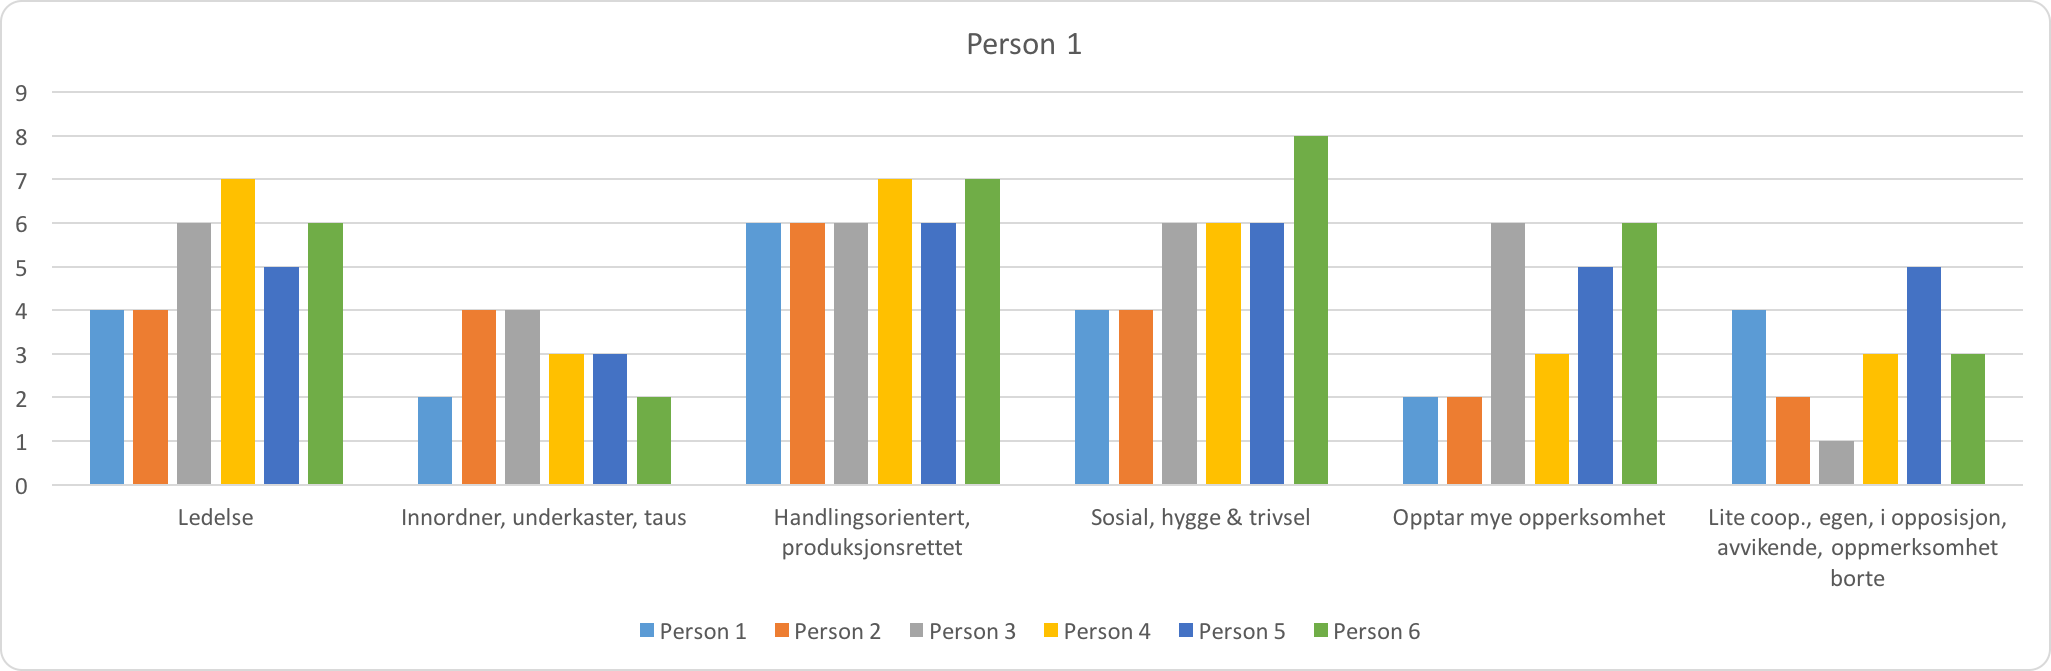
\includegraphics[width=1\textwidth]{gfx/roller_person1.png}
\caption{Roller – Person 1}
\label{roller_person1}
\end{figure}

\begin{figure}[!ht]
\centering
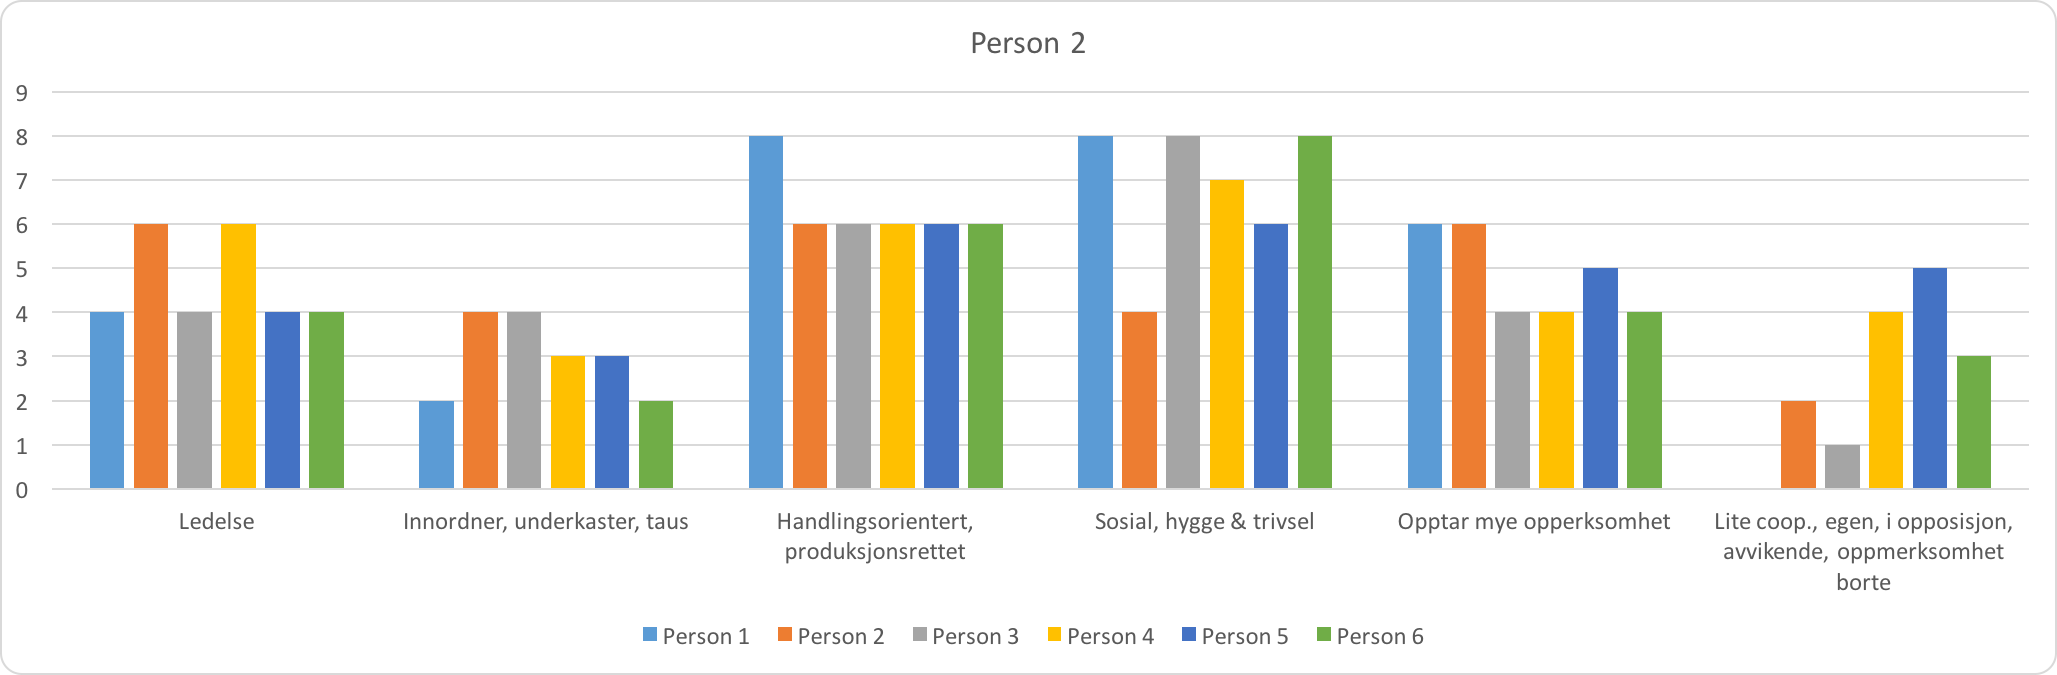
\includegraphics[width=1\textwidth]{gfx/roller_person2.png}
\caption{Roller – Person 2}
\label{roller_person2}
\end{figure}

\begin{figure}[!ht]
\centering
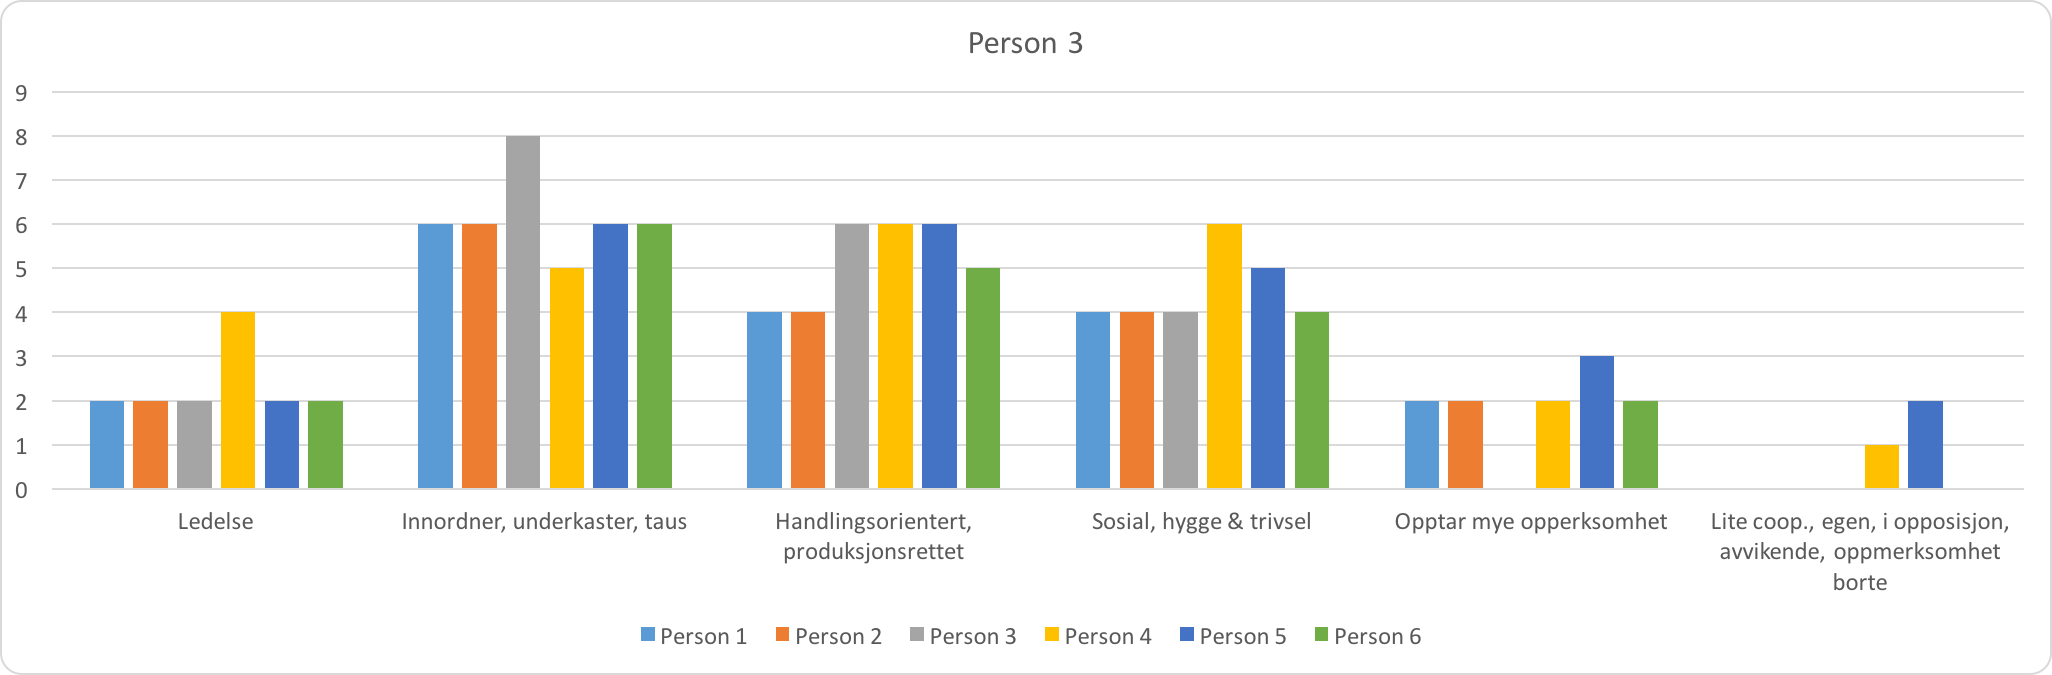
\includegraphics[width=1\textwidth]{gfx/roller_person3.png}
\caption{Roller – Person 3}
\label{roller_person3}
\end{figure}

\begin{figure}[!ht]
\centering
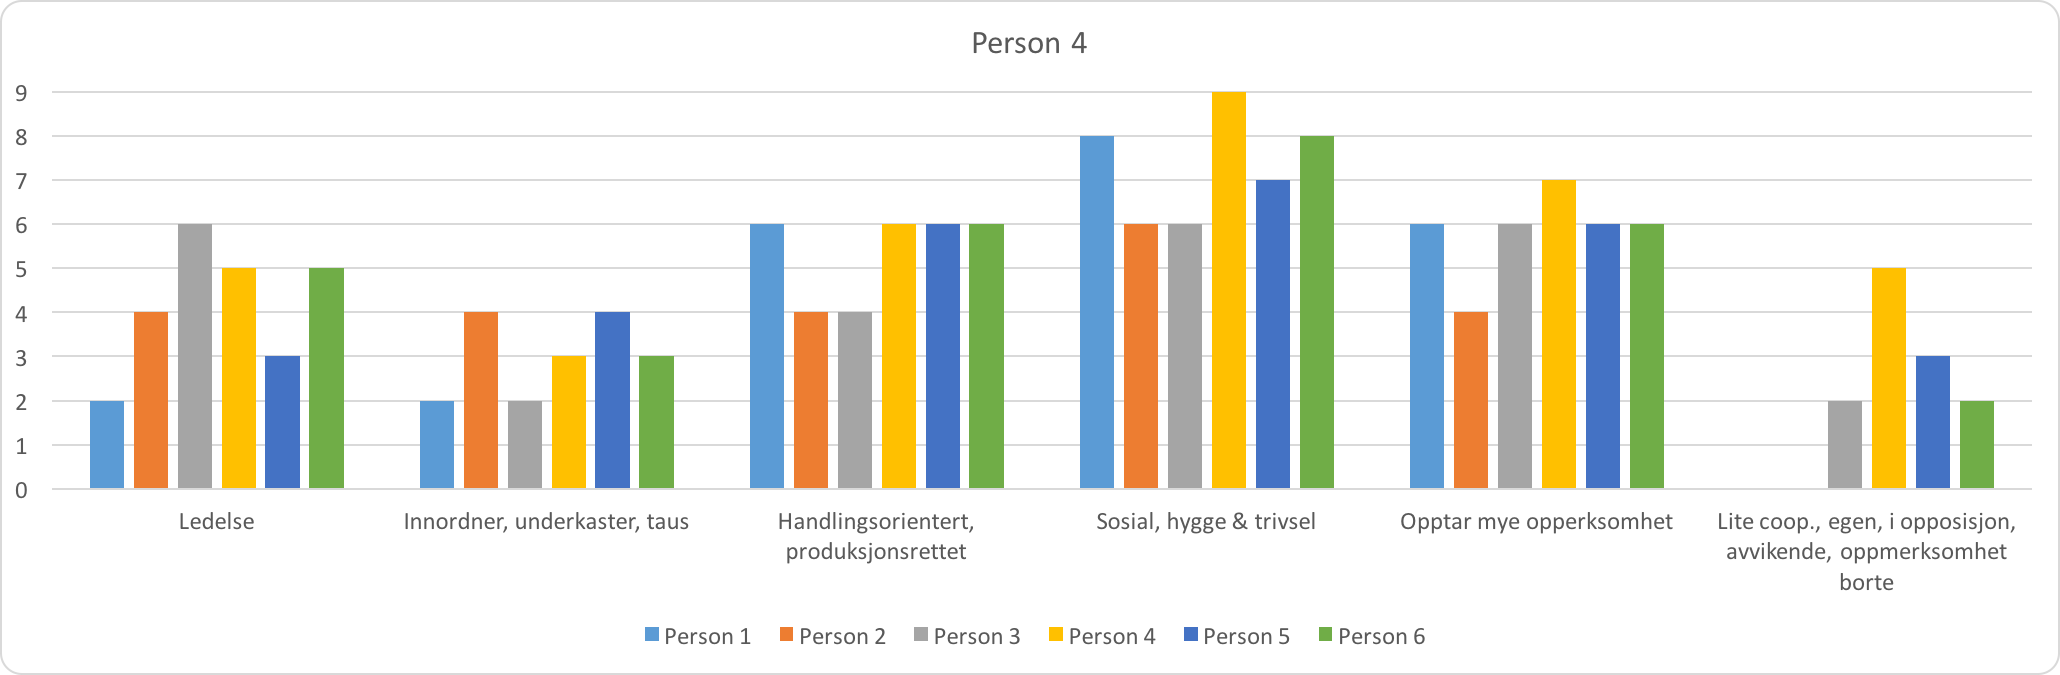
\includegraphics[width=1\textwidth]{gfx/roller_person4.png}
\caption{Roller – Person 4}
\label{roller_person4}
\end{figure}

\begin{figure}[!ht]
\centering
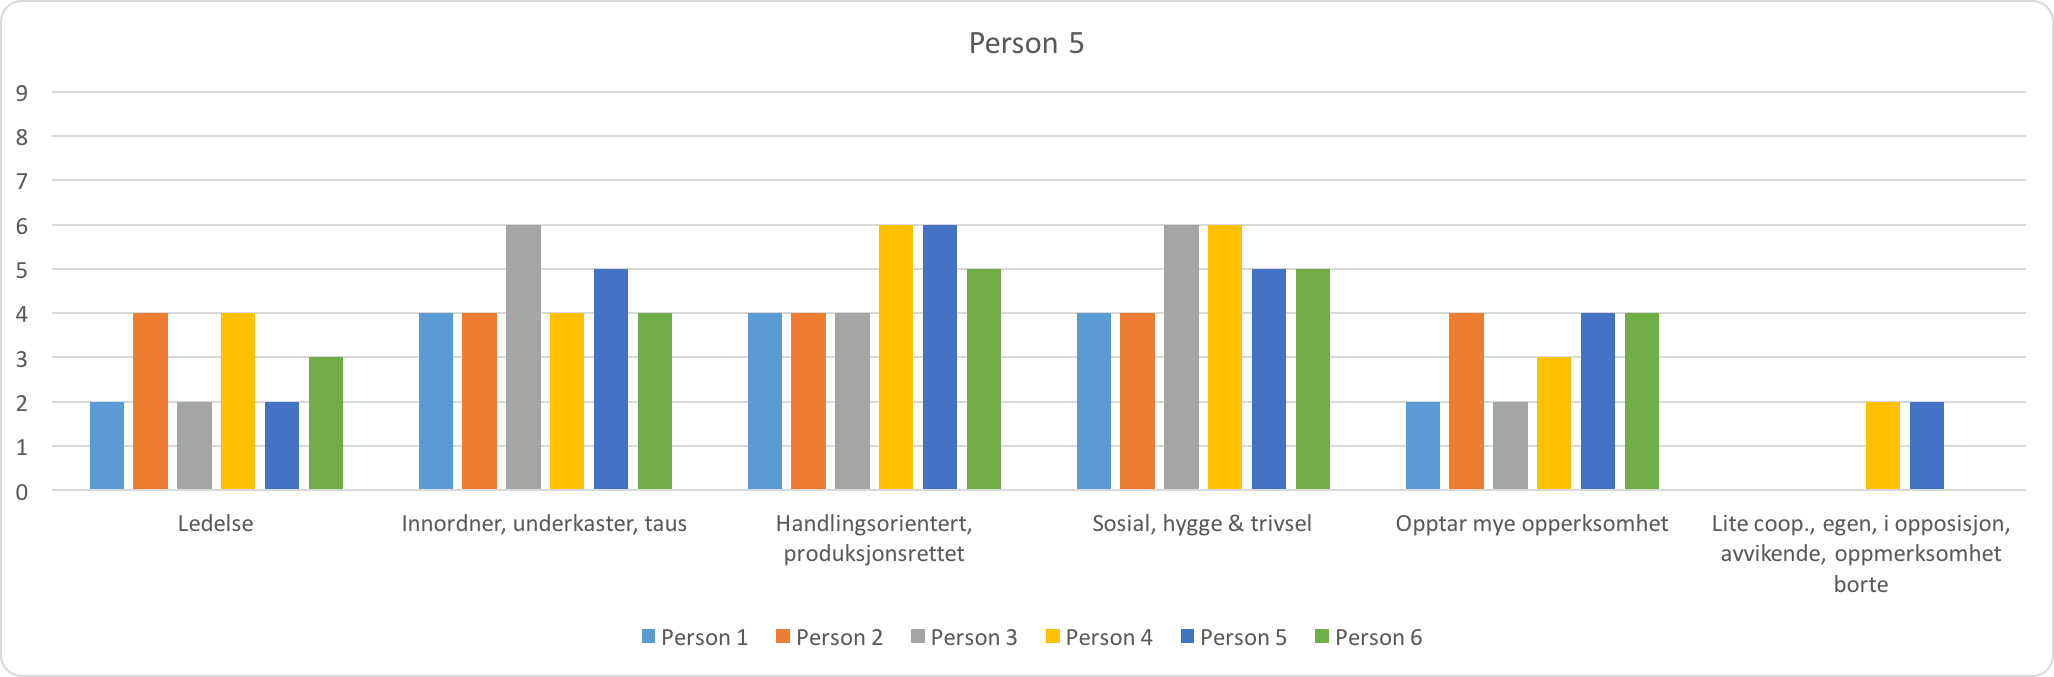
\includegraphics[width=1\textwidth]{gfx/roller_person5.png}
\caption{Roller – Person 5}
\label{roller_person5}
\end{figure}

\begin{figure}[!ht]
\centering
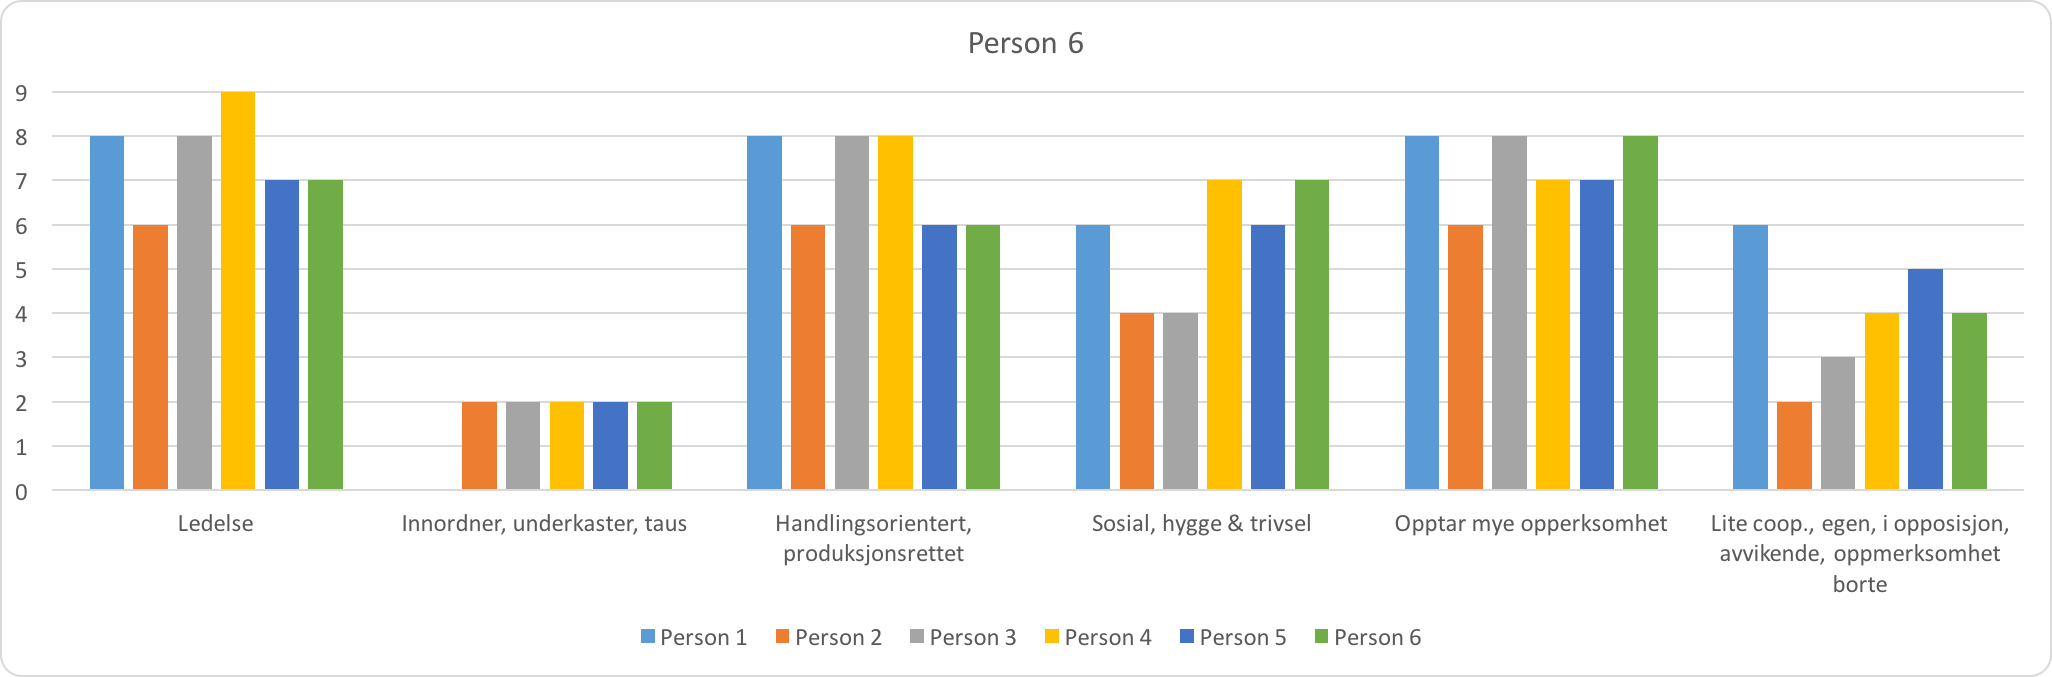
\includegraphics[width=1\textwidth]{gfx/roller_person6.png}
\caption{Roller – Person 6}
\label{roller_person6}
\end{figure}